% Options for packages loaded elsewhere
\PassOptionsToPackage{unicode}{hyperref}
\PassOptionsToPackage{hyphens}{url}
%
\documentclass[
]{article}
\usepackage{amsmath,amssymb}
\usepackage{lmodern}
\usepackage{iftex}
\ifPDFTeX
  \usepackage[T1]{fontenc}
  \usepackage[utf8]{inputenc}
  \usepackage{textcomp} % provide euro and other symbols
\else % if luatex or xetex
  \usepackage{unicode-math}
  \defaultfontfeatures{Scale=MatchLowercase}
  \defaultfontfeatures[\rmfamily]{Ligatures=TeX,Scale=1}
\fi
% Use upquote if available, for straight quotes in verbatim environments
\IfFileExists{upquote.sty}{\usepackage{upquote}}{}
\IfFileExists{microtype.sty}{% use microtype if available
  \usepackage[]{microtype}
  \UseMicrotypeSet[protrusion]{basicmath} % disable protrusion for tt fonts
}{}
\makeatletter
\@ifundefined{KOMAClassName}{% if non-KOMA class
  \IfFileExists{parskip.sty}{%
    \usepackage{parskip}
  }{% else
    \setlength{\parindent}{0pt}
    \setlength{\parskip}{6pt plus 2pt minus 1pt}}
}{% if KOMA class
  \KOMAoptions{parskip=half}}
\makeatother
\usepackage{xcolor}
\usepackage{longtable,booktabs,array}
\usepackage{calc} % for calculating minipage widths
% Correct order of tables after \paragraph or \subparagraph
\usepackage{etoolbox}
\makeatletter
\patchcmd\longtable{\par}{\if@noskipsec\mbox{}\fi\par}{}{}
\makeatother
% Allow footnotes in longtable head/foot
\IfFileExists{footnotehyper.sty}{\usepackage{footnotehyper}}{\usepackage{footnote}}
\makesavenoteenv{longtable}
\usepackage{graphicx}
\makeatletter
\def\maxwidth{\ifdim\Gin@nat@width>\linewidth\linewidth\else\Gin@nat@width\fi}
\def\maxheight{\ifdim\Gin@nat@height>\textheight\textheight\else\Gin@nat@height\fi}
\makeatother
% Scale images if necessary, so that they will not overflow the page
% margins by default, and it is still possible to overwrite the defaults
% using explicit options in \includegraphics[width, height, ...]{}
\setkeys{Gin}{width=\maxwidth,height=\maxheight,keepaspectratio}
% Set default figure placement to htbp
\makeatletter
\def\fps@figure{htbp}
\makeatother
\setlength{\emergencystretch}{3em} % prevent overfull lines
\providecommand{\tightlist}{%
  \setlength{\itemsep}{0pt}\setlength{\parskip}{0pt}}
\setcounter{secnumdepth}{5}
\usepackage{amsmath}
\usepackage{mathtools}
\ifLuaTeX
  \usepackage{selnolig}  % disable illegal ligatures
\fi
\IfFileExists{bookmark.sty}{\usepackage{bookmark}}{\usepackage{hyperref}}
\IfFileExists{xurl.sty}{\usepackage{xurl}}{} % add URL line breaks if available
\urlstyle{same} % disable monospaced font for URLs
\hypersetup{
  pdftitle={Algebraic perfect hash functions},
  pdfauthor={Alex Towell},
  hidelinks,
  pdfcreator={LaTeX via pandoc}}

\title{Algebraic perfect hash functions}
\author{Alex Towell}
\date{}

\usepackage{amsthm}
\newtheorem{theorem}{Theorem}[section]
\newtheorem{lemma}{Lemma}[section]
\newtheorem{corollary}{Corollary}[section]
\newtheorem{proposition}{Proposition}[section]
\newtheorem{conjecture}{Conjecture}[section]
\theoremstyle{definition}
\newtheorem{definition}{Definition}[section]
\theoremstyle{definition}
\newtheorem{example}{Example}[section]
\theoremstyle{definition}
\newtheorem{exercise}{Exercise}[section]
\theoremstyle{definition}
\newtheorem{hypothesis}{Hypothesis}[section]
\theoremstyle{remark}
\newtheorem*{remark}{Remark}
\newtheorem*{solution}{Solution}
\begin{document}
\maketitle

{
\setcounter{tocdepth}{2}
\tableofcontents
}
\hypertarget{algebraic-perfect-hash-functions}{%
\section{Algebraic perfect hash functions}\label{algebraic-perfect-hash-functions}}

See the \href{https://queelius.github.io/perfect_hash_functions/index.html}{function reference}

A \emph{set} is an unordered collection of distinct elements.
If we know the elements in a set are given by \(a\), \(b\), and \(c\), we may denote
the set with the notation \(\{a,c,b\}\).

A \emph{finite} set has a finite number of elements.
For example, \(\{ 1, 3, 5 \}\) is a finite set with three elements.
When sets \(\mathbb{A}\) and \(\mathbb{B}\) are \emph{isomorphic}, denoted by
\(\mathbb{A} \cong \mathbb{B}\), they can be put into a one-to-one correspondence
(bijection), e.g., \(\{b,a,c\} \cong \{1,2,3\}\).
Since there exists at least one bijection between isomorphic sets, we can
losslessly convert one to the other and thus, isomorphic sets are in some sense
equivalent.

The cardinality of a finite set \(\mathbb{A}\) is the number of elements in the
set, denoted by \(|\mathbb{A}|\), e.g., \(|\{ 1, 3, 5\}| = 3\).
A \emph{countably infinite} set is isomorphic to the set of natural numbers
\(\mathbb{N} = \{1,2,3,\ldots\}\).

Given two elements \(a\) and \(b\), an ordered pair of \(a\) then \(b\) is denoted by
\((a,b)\), where \((a,b) = (c,d)\) iff \(a = c\) and \(b = d\).
Ordered pairs are non-commutative and non-associative, i.e., \((a,b) \neq (b,a)\)
if \(a \neq b\) and \(\bigl(a,(b,c)\bigr) \neq \bigl((b,a),c\bigr)\).

Related to the ordered pair is the Cartesian product.

\begin{definition}
The set
\[
\mathbb{X} \times \mathbb{Y} \coloneqq \left\{(x,y) \colon x \in 
\mathbb{X} \land y \in \mathbb{Y}\right\}
\]
is the Cartesian product of sets \(\mathbb{X}\) and \(\mathbb{Y}\).
\end{definition}

By the non-commutative and non-associative property of ordered pairs, the
Cartesian product is non-commutative and non-associative.
However, they are isomorphic, i.e.,
\(\mathbb{X} \times \mathbb{Y} \cong \mathbb{Y} \times \mathbb{X}\).

A \emph{tuple} is a generalization of order pairs which can consist of an
arbitrary number of elements, e.g., \((x_1,x_2,\ldots,x_n)\).

\begin{definition}
The \(n\)-fold Cartesian product of sets \(\mathbb{X_1},\ldots,\mathbb{X_n}\) is
given by
\[
\mathbb{X_1} \times \cdots \times \mathbb{X_n} \coloneqq
  \bigl\{(x_1,\ldots,x_n) : x_1 \in \mathbb{X_1} \land \cdots
  \land x_n \in \mathbb{X_n}\bigr\}.
\]
\end{definition}

Note that
\[
\mathbb{X_1} \times \mathbb{X_2} \times \mathbb{X_3} \cong
  \mathbb{X_1} \times \left(\mathbb{X_2} \times \mathbb{X_3}\right) \cong
  \left(\mathbb{X_1} \times \mathbb{X_2}\right) \times \mathbb{X_3},
\]
thus we may implicitly convert between them without ambiguity.

If each set in the \(n\)-ary Cartesian product is the same, the power notation may
be used, e.g., \(\mathbb{X}^3 \equiv \mathbb{X} \times \mathbb{X} \times \mathbb{X}\).
As special cases, the \(0\)-ary (nullary) Cartesian product is defined to be
\(\{ \emptyset \}\) and the \(1\)-ary (unary) Cartesian product is the identity,
e.g., \(\mathbb{X}^1 = \mathbb{X}\).

\begin{definition}
A one-to-one relation between \(\{0,1\}^m\) and \(\{1,2,\ldots,2^m\}\) is given
by the equation
\[
b_m \Longleftrightarrow \sum_{j=1}^{m} 2^{m - j + 1} b_j\,,
\]
where \(b_m \in \{0,1\}^m\).
We denote the transformation in either direction by the unary operation \('\),
e.g., \(2' = 0\).
\end{definition}

We show some of the mappings in Table \ref{tab:convert}.

\begin{longtable}[]{@{}ll@{}}
\caption{\label{tab:convert} A one-to-one relation between \(\{0,1\}^*\) and \(\mathbb{N}\).}\tabularnewline
\toprule()
\(\mathbb{N}\) & \(\{0,1\}^*\) \\
\midrule()
\endfirsthead
\toprule()
\(\mathbb{N}\) & \(\{0,1\}^*\) \\
\midrule()
\endhead
1 & \(\emptyset\) \\
2 & \(0_2\) \\
3 & \(1_2\) \\
4 & \(00_2\) \\
5 & \(01_2\) \\
6 & \(10_2\) \\
7 & \(11_2\) \\
8 & \(000_2\) \\
9 & \(001_2\) \\
10 & \(010_2\) \\
11 & \(011_2\) \\
12 & \(100_2\) \\
13 & \(101_2\) \\
14 & \(110_2\) \\
15 & \(111_2\) \\
\(\vdots\) & \(\vdots\) \\
\bottomrule()
\end{longtable}

A \emph{hash function} is given by the following definition.

\begin{definition}
Hash functions of type \(\mathbb{X} \mapsto \mathbb{Y}\) are just total
functions, normally with a finite codomain, with the weak assumption that they
will be used as a device to assign elements from \(\mathbb{X}\) a value from
\(\mathbb{Y}\) without requiring any particular rule.
\end{definition}

For a given bit string \(x\) and hash function \(\operatorname{hash}\),
\(y = \operatorname{hash}(x)\) is denoted the \emph{hash} of \(x\).

We are particularly interested in \emph{perfect} hash functions as given by the
following definition.

\begin{definition}
A perfect hash function over the set \(\mathbb{A} \subseteq \mathbb{X}\), denoted
by
\[
\operatorname{hash}_{\mathbb{A}} \colon \mathbb{X} \mapsto \mathbb{Y},
\]
is an injective function when restricted to \(\mathbb{A}\).
That is, there are no collisions among elements of \(\mathbb{A}\),
\(\operatorname{hash}_{\mathbb{A}}(x) \neq \operatorname{hash}_{\mathbb{A}}(y)\)
for all \(x, y \in \mathbb{A}\), \(x \neq y\).
\end{definition}

Perfect hash functions are generally \emph{surjective} when not restricted to
the range of elements it perfectly hashes.

The \emph{load factor} is given by the following definition.

\begin{definition}[Load factor]
\label{def:loadfactor}
The proportion of hashes mapped to by
\(\operatorname{hash}_{\mathbb{A}} \colon \mathbb{X} \mapsto \mathbb{N}\) over
subset \(\mathbb{A}\) is denoted the load factor.
Specifically, the load factor of \(\operatorname{hash}_{\mathbb{A}}\) is a rational number given
by
\[
\frac{|\operatorname{hash}_{\mathbb{A}}(\mathbb{A})|}
  {|{\operatorname{image}(\operatorname{hash}_{\mathbb{A}})}|}.
\]
\end{definition}

A \emph{minimal} perfect hash has a load factor \(1\).

A perfect hash function of type \(\mathbb{X} \mapsto \mathbb{Y}\) over
\(\mathbb{A}\) with a load factor \(r\) may be denoted by
\(\operatorname{hash}_{\mathbb{A}}^{r}\).
If \(m = |\{\mathbb{A}\}|\) and we are interested in drawing attention to the
cardinality of the perfect hash function, we may also denote it by
\(\operatorname{hash}_{m}^{r}\).

\begin{figure}
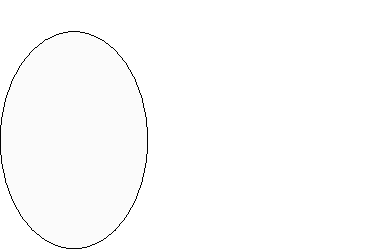
\includegraphics[width=0.7\linewidth]{img/pf} \caption{This is a figure caption.}\label{fig:ho-plot}
\end{figure}

Every hash function in \(\mathbb{X} \mapsto \mathbb{Y}\) is a perfect hash
function over some subset of \(\mathbb{X}\), e.g., every hash function is
trivially a perfect hash function of the empty set and singleton sets.

Assuming \(\mathbb{X}\) and \(\mathbb{Y}\) are finite, the set of hash functions of
type \(\mathbb{X} \mapsto \mathbb{Y}\), which may also be denoted by
\(\mathbb{Y}^{\mathbb{X}}\), has a cardinality
\[
|{\mathbb{Y}}|^{|\mathbb{X}|}.
\]
The set of perfect hash functions over \(\mathbb{A} \subseteq \mathbb{X}\) is a
subset of \(\mathbb{X} \mapsto \mathbb{Y}\) with the predicate that no collisions
may occur on any pair of elements in \(\mathbb{A}\).

\end{document}
